\documentclass[aspectratio=169,11pt]{beamer}
\usepackage{assets/acemoglu-beamer}
\title[AKO (2026): auditoría]{AI, Human Cognition and Knowledge Collapse}
\subtitle{Pregunta, mecanismo, bienestar y una objeción de robustez}
\author{Belén Vásquez}\institute{Universidad del Pacífico}\date{Septiembre de 2026}
\begin{document}
\begin{frame}[plain]\titlepage\vspace{-1em}\begin{center}\small\paperref\\[.4em]\href{\RepoURL}{\texttt{github.com/sbvasquezg-ux/ai-04-acemoglu}}\end{center}\end{frame}

\begin{frame}{1 \textperiodcentered{} Pregunta y problema del agente}
\footnotesize
\textbf{Objetivo.} Explicar por qué una IA más precisa puede reducir el esfuerzo humano y, con él, el conocimiento general que beneficia a todos.
\[
\max_{e\ge0}\ U=f(0,0)+G(X)\Delta_G+G(X)G(Y)\Delta_X-\frac{e^\alpha}{\alpha},
\quad Y=\sigma^{-2}+\lambda_Ie+\tau_A.
\]
\[
\underbrace{\Delta_XG(X)\lambda_Ig(Y)}_{MB(e;X,\tau_A)}=e^{\alpha-1}.
\]
\begin{itemize}\item $e$: esfuerzo cognitivo; $X$: precisión del conocimiento general heredado; $Y$: precisión contextual total.
\item $\tau_A$: precisión del consejo de IA; $\lambda_Ie$: precisión creada por el esfuerzo; $\alpha>1$: curvatura del costo.
\item $G(z)$: probabilidad de decidir correctamente con precisión $z$; $g(z)=G'(z)>0$.
\end{itemize}
\keybox{\textbf{Mecanismo:} $X$ eleva el beneficio marginal de pensar; $\tau_A$ mejora $Y$ sin esfuerzo y reduce ese beneficio. El agente no internaliza que su esfuerzo también alimenta el conocimiento público futuro.}
\sourcefoot{PDF 20-02-2026, §§3.1--3.5, pp. 8--15; ecuaciones (4)--(6).}
\end{frame}

\begin{frame}{2 \textperiodcentered{} Observación 1: complemento y sustituto}
\footnotesize
\textbf{Condiciones:} señales gaussianas independientes, $\lambda_I>0$, costo $e^\alpha/\alpha$ con $\alpha>1$, $\Delta_I=0$, $\Delta_X>0$ y solución interior con $X,Y>0$.
\[
U_{eX}=\Delta_X\lambda_Ig(X)g(Y)>0,
\qquad U_{e\tau_A}=\Delta_XG(X)\lambda_Ig'(Y)<0.
\]
\begin{block}{Lectura económica}
$U_{eX}>0$: más conocimiento general aumenta el retorno de una hora adicional de esfuerzo. $U_{e\tau_A}<0$: una recomendación más precisa reduce ese retorno porque ya aporta precisión contextual. Con costo convexo, $e_X^*>0$ y $e_{\tau_A}^*<0$.
\end{block}
\keybox{\textbf{Por qué importa:} menos $e$ hoy implica menos señal pública agregada y menor $X$ mañana. La observación estática abre el canal dinámico del colapso. En $X=0$, sin embargo, $e^*=0$ y la desigualdad estricta deja de estar bien definida.}
\sourcefoot{§§3.4--3.5, pp. 13--15; Observaciones 1--2 y nota 4.}
\end{frame}

\begin{frame}{3 \textperiodcentered{} Bienestar: cómo leer el gráfico}
\scriptsize
\vspace{-.35em}
\[
\frac{\partial\bar U^+}{\partial\tau_A}=
\underbrace{g(\bar Y_h)G(\bar X_h)\Delta_X}_{DE\ge0}
+\underbrace{\frac{\partial G(\bar X_h)}{\partial\tau_A}[\Delta_G+G(\bar Y_h)\Delta_X]}_{-IE\le0}.
\]
\begin{columns}[T,onlytextwidth]
\column{.57\textwidth}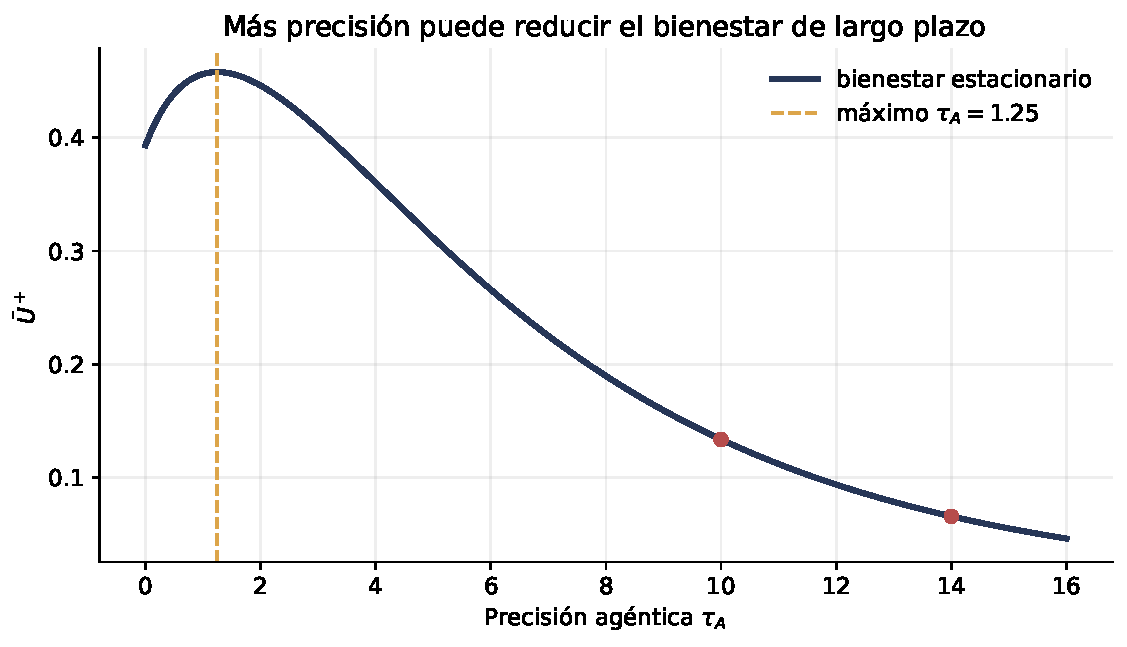
\includegraphics[width=\linewidth,height=.43\textheight,keepaspectratio]{extra/figures/welfare-accuracy.pdf}
\column{.40\textwidth}
\begin{itemize}\item \textbf{Eje $x$:} $\tau_A$, precisión exógena de la recomendación de IA. Moverse a la derecha significa mejor consejo.
\item \textbf{Eje $y$:} $\bar U^+$, utilidad neta en el estado estacionario alto.
\item \textbf{Tramo ascendente:} domina el efecto directo de acertar más hoy.
\item \textbf{Tramo descendente:} domina la pérdida de $X$ causada por menor esfuerzo y agregación.
\end{itemize}
\end{columns}
\keybox{\textbf{Interpretación:} curva de U invertida. El bienestar sube hasta $\tau_A^\star$ y luego cae estrictamente. No mide utilidad descontada ni distribución.}
\sourcefoot{Ecuación (10), §4.3 y Proposiciones 10--11, pp. 24--27; cálculo propio.}
\end{frame}

\begin{frame}{4 \textperiodcentered{} Objeción: el cero exacto depende del baseline}
\footnotesize
\begin{columns}[T,onlytextwidth]
\column{.61\textwidth}
\textbf{Qué cuestiono.} El paper demuestra que $\bar X=0$ puede ser absorbente, pero ese resultado necesita simultáneamente:
\begin{enumerate}\item $\Delta_I=0$: el conocimiento específico solo no produce valor.
\item $\tau_{syn}=0$: la IA no crea un flujo autónomo de conocimiento general.
\item Agentes atomísticos y homogéneos: nadie internaliza la externalidad y no quedan especialistas activos.
\end{enumerate}
\textbf{Relajaciones:} con $\tau_{syn}>0$, $F_{syn}(0)>0$ (Prop. 15); con $\Delta_I>0$, pensar conserva retorno privado en $X=0$. Quispe--Xu aporta evidencia compatible con aprendizaje al usar IA, otro canal que preservaría capacidad humana.
\keybox{\textbf{Veredicto.} Sí sobrevive el riesgo de una economía con poco conocimiento general. La desaparición exacta requiere condiciones de filo de navaja; el resultado robusto es ``conocimiento bajo'', no necesariamente cero.}
\column{.35\textwidth}
\begin{center}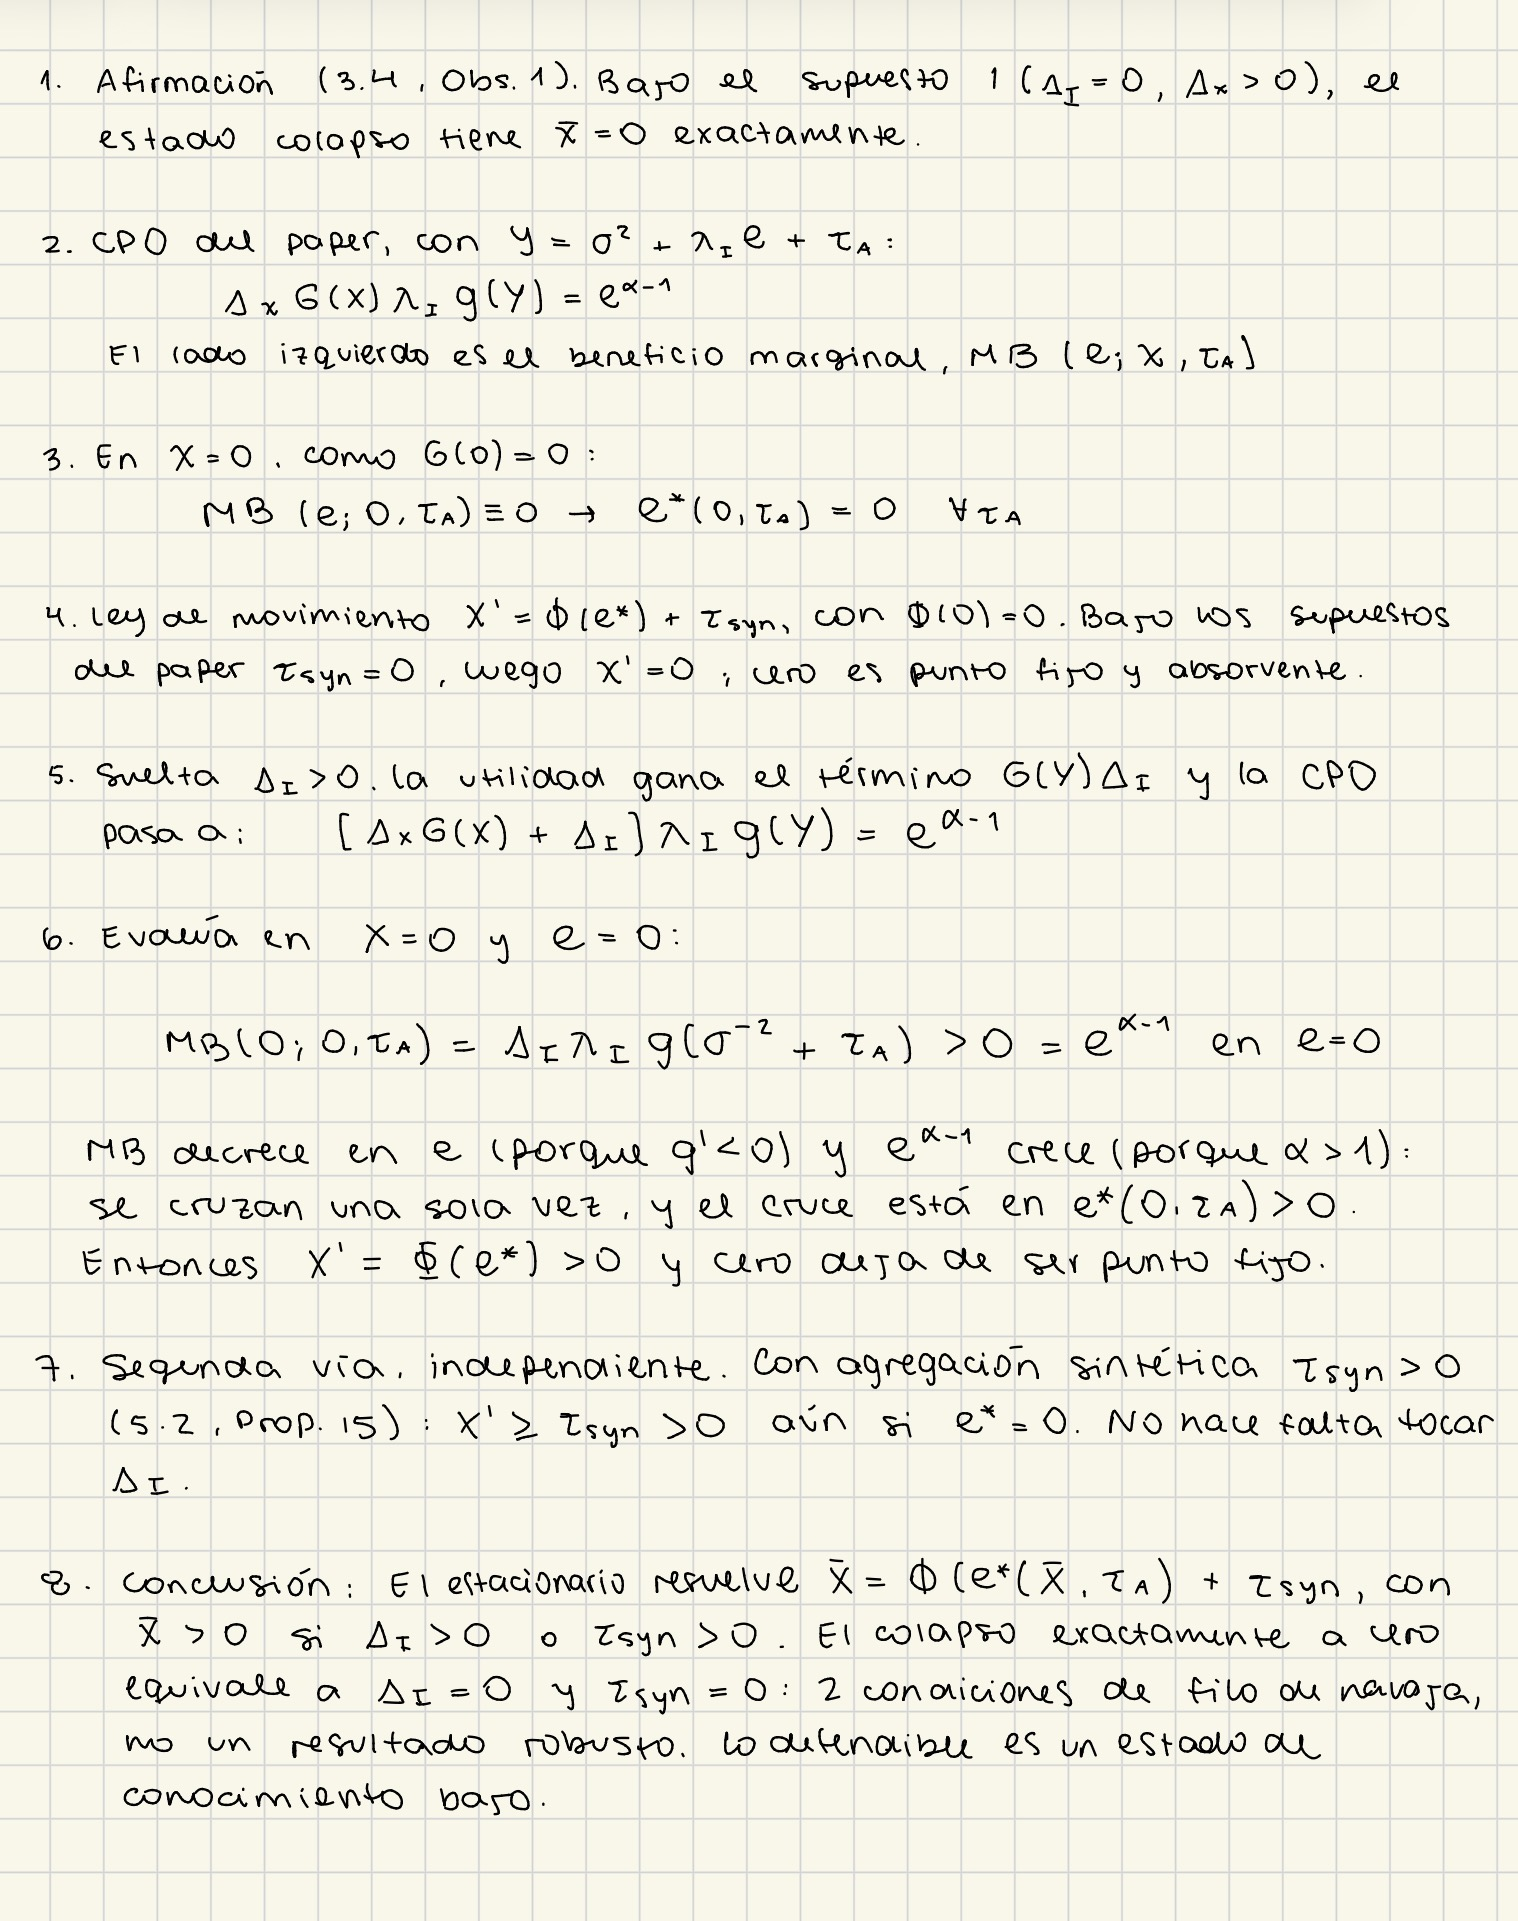
\includegraphics[width=\linewidth,height=.54\textheight,keepaspectratio]{hand/manual-verification.jpg}\\[-.2em]\scriptsize Verificación manuscrita aportada por la estudiante.\end{center}
\end{columns}
\sourcefoot{§§5.1--5.2, pp. 30--32; Assumption 1, p. 9; hand/README.md.}
\end{frame}
\end{document}
